\documentclass[a4paper,12pt,obeyspaces,spaces,hyphens]{article}

\def \trainingtitle{Yocto Project and OpenEmbedded development training}
\def \trainingduration{On-site training, 3 days}
\def \agendalanguage{english}
\def \training{yocto}

\usepackage{agenda}

\begin{document}

\feshowtitle

\feagendasummaryitem{Title}{
  {\bf \trainingtitle{}}
}
\feagendasummaryitem{Training objectives}{
  \begin{itemize}
  \item Be able to understand the role and principle of an embedded
    Linux build system, and compare Yocto Project/OpenEmbedded to
    other tools offering similar functionality.
  \item Be able to configure and build basic embedded Linux system
    with Yocto, and install the result on an embedded platform.
  \item Be able to write and extend recipes, for your own packages or
    customizations.
  \item Be able to use existing layers of recipes, and create your own
    new layers.
  \item Be able to integrate support for your own embedded board into
    a BSP layer.
  \item Be able to create custom images.
  \item Be able to use the tools and workflows suitable to develop
    applications with the Yocto Project SDK.
  \end{itemize}
}
\feagendasummaryitem{Duration}{
  {\bf Three} days - 24 hours (8 hours per day).
}
\onsitepedagogics{40}{60}{yocto}
\feagendasummaryitem{Trainer}{
  One of the engineers listed on
  \newline \url{https://bootlin.com/training/trainers/}
}
\feagendasummaryitem{Language}{
  Oral lectures: English, French.
  \newline Materials: English.
}
\feagendasummaryitem{Audience}{
  Companies and engineers interested in using
  the Yocto Project to build their embedded Linux system.
}
\feagendasummaryitem{Prerequisites}{
  \begin{itemize}
    \prerequisitecommandline
    \prerequisiteembeddedlinux
    \prerequisiteenglish
  \end{itemize}
}
\ferequiredequipmentonsite{}
\certificate{}
\disabilities{}

\feagendatwocolumn
{Hardware, first option}
{
  BeagleBone Black board
  \begin{itemize}
  \item An ARM AM335x processor from Texas Instruments (Cortex-A8
    based), 3D acceleration, etc.
  \item 512 MB of RAM
  \item 2 GB of on-board eMMC storage
        \newline(4 GB in Rev C)
  \item USB host and device
  \item HDMI output
  \item 2 x 46 pins headers, to access UARTs, SPI buses, I2C buses
    and more.
  \end{itemize}
  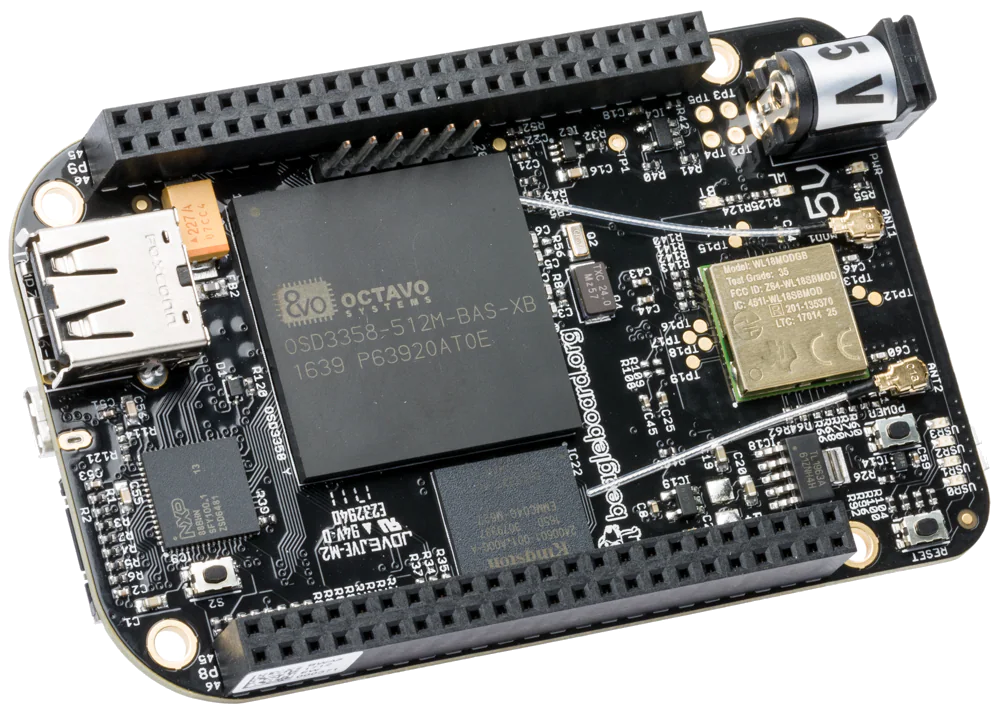
\includegraphics[width=5cm]{../slides/beagleboneblack-board/beagleboneblack.png}
}
{Hardware, second option}
{
  STMicroelectronics STM32MP157D-DK1 Discovery board
  \begin{itemize}
  \item STM32MP157D (dual Cortex-A7) CPU from STMicroelectronics
  \item USB powered
  \item 512 MB DDR3L RAM
  \item Gigabit Ethernet port
  \item 4 USB 2.0 host ports
  \item 1 USB-C OTG port
  \item 1 Micro SD slot
  \item On-board ST-LINK/V2-1 debugger
  \item Arduino Uno v3-compatible headers
  \item Audio codec
  \item Misc: buttons, LEDs
  \end{itemize}
  \includegraphics[width=5cm]{../slides/discovery-board-dk1/discovery-board-dk1.png}
}

\section{Day 1 - Morning}

\feagendaonecolumn
{Lecture - Introduction to embedded Linux build systems}
{
  \begin{itemize}
  \item Overview of an embedded Linux system architecture
  \item Methods to build a root filesystem image
  \item Usefulness of build systems
  \end{itemize}
}
\\
\feagendatwocolumn
{Lecture - Overview of the Yocto Project and the Poky reference system}
{
  \begin{itemize}
  \item Organization of the project source tree
  \item Building a root filesystem image using the Yocto Project
  \end{itemize}
}
{Lab - First Yocto Project build}
{
  \begin{itemize}
  \item Downloading the Poky reference build system
  \item Building a system image
 \end{itemize}
}

\section{Day 1 - Afternoon}
\feagendatwocolumn
{Lecture - Using Yocto Project - basics}
{
  \begin{itemize}
  \item Organization of the build output
  \item Flashing and installing the system image
  \end{itemize}
}
{Lab - Flashing and booting}
{
  \begin{itemize}
  \item Flashing and booting the image on the board
  \end{itemize}
}

\feagendatwocolumn
{Lecture - Using Yocto Project - advanced usage}
{
  \begin{itemize}
  \item Configuring the build system
  \item Customizing the package selection
  \end{itemize}
}
{Lab - Using NFS and configuring the build}
{
  \begin{itemize}
  \item Configuring the board to boot over NFS
  \item Learn how to use the \code{PREFERRED_PROVIDER} mechanism
  \end{itemize}
}
\\
\section{Day 2 - Morning}

\feagendatwocolumn
{Lecture - Writing recipes - basics}
{
  \begin{itemize}
  \item Writing a minimal recipe
  \item Adding dependencies
  \item Development workflow with {\em bitbake}
  \end{itemize}
}
{Lab - Adding an application to the build}
{
  \begin{itemize}
  \item Writing a recipe for {\em nInvaders}
  \item Adding {\em nInvaders} to the final image
  \end{itemize}
}

\feagendaonecolumn
{Lecture - Writing recipes - advanced features}
{
  \begin{itemize}
  \item Extending and overriding recipes
  \item Adding steps to the build process
  \item Learn about classes
  \item Analysis of examples
  \item Logging
  \item Debugging dependencies
  \end{itemize}
}

\section{Day 2 - Afternoon}

\feagendaonecolumn
{Lab - Learning how to configure packages}
{
  \begin{itemize}
  \item Extending a recipe to add configuration files
  \item Using \code{ROOTFS_POSTPROCESS_COMMAND} to modify the final rootfs
  \item Studying package dependencies
  \end{itemize}
}
\feagendatwocolumn
{Lecture - Layers}
{
  \begin{itemize}
  \item What layers are
  \item Where to find layers
  \item Creating a layer
  \end{itemize}
}
{Lab - Writing a layer}
{
  \begin{itemize}
  \item Learn how to write a layer
  \item Add the layer to the build
  \item Move {\em nInvaders} to the new layer
  \end{itemize}
}

\section{Day 3 - Morning}

\feagendatwocolumn
{Lecture - Writing a BSP}
{
  \begin{itemize}
  \item Extending an existing BSP
  \item Adding a new machine
  \item Bootloaders
  \item Linux and the linux-yocto recipe
  \item Adding a custom image type
  \end{itemize}
}
{Lab - Implementing the kernel changes}
{
  \begin{itemize}
  \item Extend the kernel recipe to add the nunchuk driver
  \item Configure the kernel to compile the nunchuk driver
  \item Play {\em nInvaders}
  \end{itemize}
}

\section{Day 3 - Afternoon}

\feagendatwocolumn
{Lecture - Creating a custom image}
{
  \begin{itemize}
  \item Writing an image recipe
  \item Adding users/groups
  \item Adding custom configuration
  \item Writing and using package groups recipes
  \end{itemize}
}
{Lab - Creating a custom image}
{
  \begin{itemize}
  \item Writing a custom image recipe
  \item Adding {\em nInvaders} to the custom image
  \end{itemize}
}
\feagendatwocolumn
{Lecture - Creating and using an SDK}
{
  \begin{itemize}
  \item Understanding the purpose of an SDK for the application
    developer
  \item Building an SDK for the custom image
  \end{itemize}
}
{Lab - Experimenting with the SDK}
{
  \begin{itemize}
  \item Building an SDK
  \item Using the Yocto Project SDK
  \end{itemize}
}

\end{document}

